\chapter{Evaluation}\label{chap:test}
After producing the application described in Chapter~\ref{chap:imp}, referring
back to the design specifications to determine its performance against the
stated criteria was the next step.  

\section{Methodology}
Using a sample of e-mails provided by my supervisor, each of them was run
through the final version of the program, and scored based on the following
attributes:

\begin{itemize}
\item Let $M$ be the total number of received fields.
\item Let $N$ be the total number of other fields.
\item 1 point is added to the total $R$ for each piece of information found in a Received field for the following:
\begin{itemize}
\item{One of device name \emph{or} IP address}
\item{Software \emph{or} protocol used}
\item{Vulnerabilities found for the relevant piece of software}
\item{Location Data}
\end{itemize}
\item 1 point is addded to $F$ for each piece of information found in other fields.
\end{itemize}

The final score for an e-mail is given as \[\frac12\left(\frac R{4M}+\frac
FN\right)\]to give a value between 0 and 1 for each e-mail.

The e-mails received have been numbered from 1 up to 70, and a random sample of
size 30 was selected using the following code:

\begin{verbatim}
>>> random.seed()
>>> random.sample(list(range(1,70)), 30)
[64, 48, 11, 21, 63, 68, 27, 69, 29,  8, 28,
 34, 13, 57, 10,  3, 22, 32, 23, 49, 26, 45,
 19,  1, 36, 46, 41, 18, 20, 17]
\end{verbatim}

Thus giving a sorted list of the following e-mails: 1, 3, 8, 10, 11, 13, 17,
18, 19, 20, 21, 22, 23, 26, 27, 28, 29, 32, 34, 36, 41, 45, 46, 48, 49, 57, 63,
64, 68, 69.

\section{Sample Output}

The following pages show the results of running the completed software on a
sample e-mail sent from my own Oxford e-mail account to my G-Mail account, the
contents of which is listed in Fragment~\ref{eg:11}.  The full table of CVE
entries is elided for brevity.  The entries in \colorbox{red!30}{this colour}
are associated with points scored for $R$, and the entries in
\colorbox{blue!30}{this colour} are associated with points scored for $F$.

\begin{example}[caption=Sample E-Mail,label=eg:11]
Delivered-To: joshuaclark94@gmail.com
Received: by |\colorbox{red!30}{10.28.1.200}| with |\colorbox{red!30}{SMTP}| id 191csp811296wmb;
        Sun, 22 May 2016 09:55:48 -0700 (PDT)
X-Received: by |\colorbox{red!30}{10.28.54.204}| with |\colorbox{red!30}{SMTP}| id y73mr6213044wmh.59.1463936148370;
        Sun, 22 May 2016 09:55:48 -0700 (PDT)
Return-Path: <joshua.clark@st-annes.ox.ac.uk>
Received: from |\colorbox{red!30}{relay14.mail.ox.ac.uk}| (relay14.mail.ox.ac.uk. [|\colorbox{red!30}{163.1.2.162}|])
        by |\colorbox{red!30}{mx.google.com}| with |\colorbox{red!30}{ESMTPS}| id mw4si38680863wjb.85.2016.05.22.09.55.48
        for <joshuaclark94@gmail.com>
        (version=TLS1_2 cipher=AES128-SHA bits=128/128);
        Sun, 22 May 2016 09:55:48 -0700 (PDT)
Received-SPF: pass (google.com: best guess record for domain of joshua.clark@st-annes.ox.ac.uk designates 163.1.2.162 as permitted sender) client-ip=163.1.2.162;
Authentication-Results: mx.google.com;
       spf=pass (google.com: best guess record for domain of joshua.clark@st-annes.ox.ac.uk designates 163.1.2.162 as permitted sender) smtp.mailfrom=joshua.clark@st-annes.ox.ac.uk
Received: from |\colorbox{red!30}{smtp4.mail.ox.ac.uk}| ([|\colorbox{red!30}{129.67.1.207}|])
	by |\colorbox{red!30}{relay14.mail.ox.ac.uk}| with |\colorbox{red!30}{esmtp (Exim 4.80)}|
	(envelope-from <joshua.clark@st-annes.ox.ac.uk>) id 1b4WfM-0003l5-jc
	for joshuaclark94@gmail.com; Sun, 22 May 2016 17:55:48 +0100
Received: from |\colorbox{red!30}{chap05.pmb.ox.ac.uk}| ([|\colorbox{red!30}{129.67.89.5}|])
	by |\colorbox{red!30}{smtp4.mail.ox.ac.uk}| with |\colorbox{red!30}{esmtp (Exim 4.80)}|
	(envelope-from <joshua.clark@st-annes.ox.ac.uk>) id 1b4WfM-0008Mz-D6
	for joshuaclark94@gmail.com; Sun, 22 May 2016 17:55:48 +0100
|\colorbox{blue!30}{X-Oxford-Username: sann4425}|
To: joshuaclark94@gmail.com
From: |\colorbox{blue!30}{Joshua Clark}| <joshua.clark@|\colorbox{blue!30}{st-annes.ox.ac.uk}|>
Subject: Test
Message-ID: <0d2bc153-4b20-8f0e-e137-804305c28527@st-annes.ox.ac.uk>
Date: Sun, 22 May 2016 18:55:16 +0100
|\colorbox{blue!30}{User-Agent}|: Mozilla/5.0 (X11; Linux x86_64; rv:45.0) Gecko/20100101
 Thunderbird/45.1.0
MIME-Version: 1.0
Content-Type: text/plain; charset=utf-8; format=flowed
Content-Transfer-Encoding: 7bit

Test
\end{example}

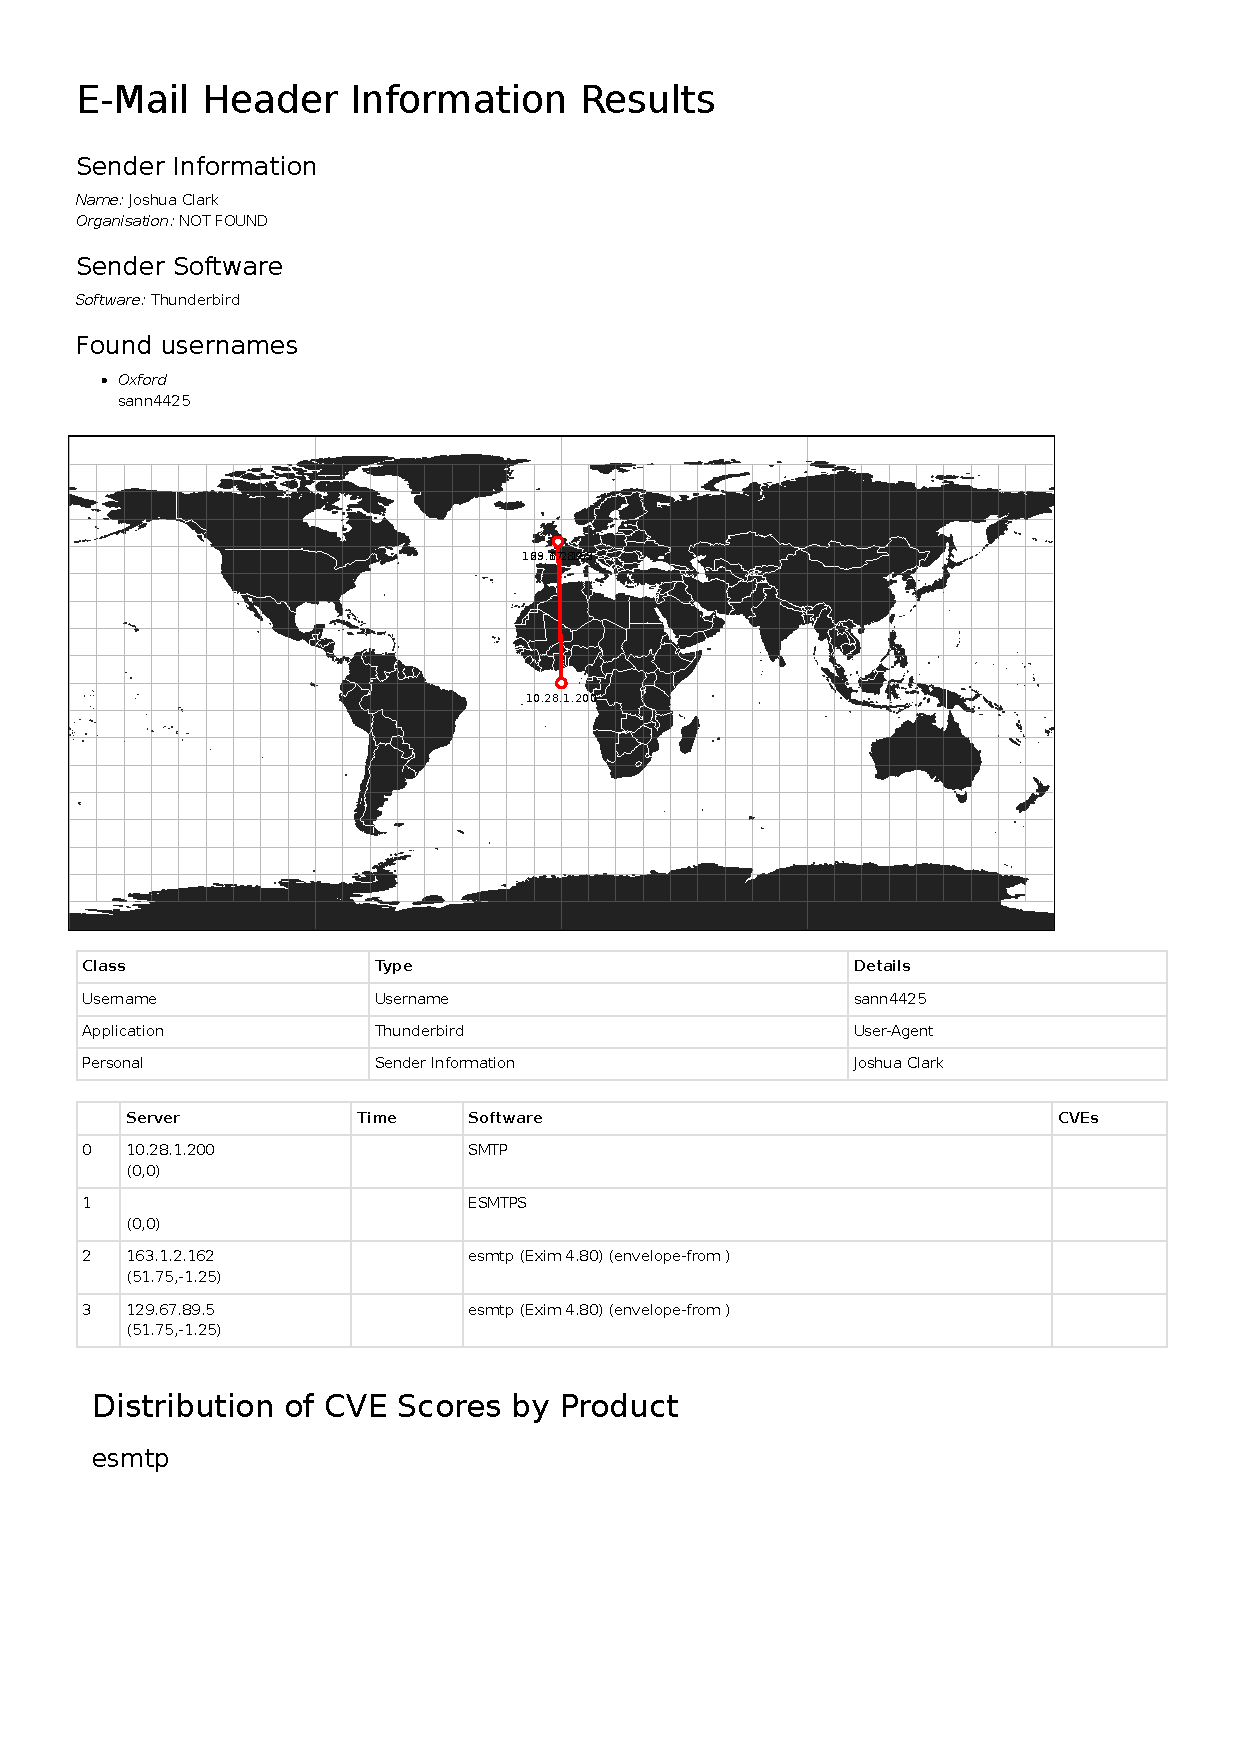
\includepdf[pages={1,2}]{test_results.pdf}

The servers highlighted in red, with the exception of the field labelled
\texttt{X-Received} have all be parsed properly, and their details collected.

No IP address is available for the \url{mx.google.com} server entry, and
therefore no location data can be found, with later locations then being
internal addresses, which also have no available location data.  However,
all of the Oxford based entries have correctly been identified as shown 
on the map.  Due to the limitations of the location data provided, it has 
not been possible to position them accurately relative to each other.

All the available software entries have been correctly detected (SMTP, ESMTP
and Thunderbird), and CVE data has been found for these pieces of software.

Lastly, my Oxford username has been correctly identified within the e-mail.

\section{Results}

Table~\ref{tab:sammn} gives the $M$ and $N$ values for the different sampled
e-mails.  These were sampled using standard Unix tools: \texttt{grep}ping for
fields and counting the output. The results for $R$ and $F$ have been listed
after completing the testing, after counting the number of entries in the final
visualisation.

\begin{table}
\centering
\begin{tabular}{@{}lrrrrrr@{}}
\toprule
Header & Total Fields &                  $M$  & $N$  & $R$ & $F$ & $S$ \\ \midrule
1.txt  & 26           & 7                     & 19   & 23  & 7   & 0.594924812    \\
3.txt  & 32           & 6                     & 26   & 16  & 6   & 0.4487179487   \\
8.txt  & 34           & 8                     & 26   & 30  & 6   & 0.5841346154   \\
10.txt & 22           & 3                     & 19   & 9   & 7   & 0.5592105263   \\
11.txt & 29           & 6                     & 23   & 23  & 6   & 0.6096014493   \\
13.txt & 17           & 4                     & 13   & 13  & 5   & 0.5985576923   \\
17.txt & 27           & 6                     & 21   & 22  & 6   & 0.6011904762   \\
18.txt & 20           & 6                     & 14   & 23  & 5   & 0.6577380952   \\
19.txt & 20           & 6                     & 14   & 21  & 4   & 0.5803571429   \\
20.txt & 22           & 7                     & 15   & 25  & 7   & 0.6797619048   \\
21.txt & 22           & 6                     & 16   & 23  & 5   & 0.6354166667   \\
22.txt & 22           & 6                     & 16   & 22  & 6   & 0.6458333333   \\
23.txt & 26           & 6                     & 20   & 20  & 7   & 0.5373563218   \\
26.txt & 19           & 6                     & 13   & 21  & 5   & 0.6298076923   \\
27.txt & 21           & 1                     & 20   & 2   & 8   & 0.45           \\
28.txt & 22           & 6                     & 16   & 23  & 4   & 0.6041666667   \\
29.txt & 20           & 6                     & 14   & 21  & 6   & 0.6517857143   \\
32.txt & 24           & 6                     & 18   & 20  & 3   & 0.5            \\
34.txt & 23           & 5                     & 18   & 19  & 4   & 0.586111111    \\
36.txt & 26           & 6                     & 20   & 21  & 4   & 0.5375         \\
41.txt & 21           & 6                     & 15   & 20  & 5   & 0.5833333333   \\
45.txt & 23           & 6                     & 17   & 22  & 5   & 0.6053921569   \\
46.txt & 26           & 5                     & 21   & 15  & 7   & 0.5416666667   \\
48.txt & 25           & 6                     & 19   & 22  & 6   & 0.6162280702   \\
49.txt & 21           & 6                     & 15   & 22  & 3   & 0.5583333333   \\
57.txt & 28           & 6                     & 22   & 21  & 4   & 0.5284090909   \\
63.txt & 23           & 5                     & 18   & 18  & 5   & 0.5888888889   \\
64.txt & 36           & 9                     & 27   & 31  & 6   & 0.5416666667   \\
68.txt & 21           & 6                     & 15   & 20  & 5   & 0.5833333333   \\
69.txt & 22           & 6                     & 16   & 21  & 5   & 0.59375        \\ \midrule
\emph{Average} & 24.3 & 5.8                   & 18.5 & 20.3& 5.4 & 0.582916135    \\ \bottomrule
\end{tabular}
\caption{$M$, $N$, $R$, $F$ and score values for chosen headers}
\label{tab:sammn}
\end{table}

\begin{figure}
	\centering\resizebox{0.75\textwidth}{!}{
\begin{tikzpicture}
\begin{axis}[
    ybar,
    ymin=0
]
\addplot +[
    hist={
        bins=10,
        data min=0.4,
        data max=0.7
    }   
] table [y index=0] {data.csv};
\end{axis}
\end{tikzpicture}}
\caption{Distribution of scores from e-mails}\label{fig:dis}
\end{figure}

The final score for the e-mails gives a minimum value of 0.449 and a maximum
value of 0.680, with an average of 0.583 and standard deviation of 0.0540. The
histogram in Figure~\ref{fig:dis} shows the distribution of scores from the
e-mails, showing a skew towards higher scores.  This is a promising result,
however, most of the score is contributed to by the trace-fields, with the 
value of $R/4N$ being consistently around 0.85.  As the aim of this project
has both focused on the disclosure of individual's data and of network
vulnerabilities, the high score from the trace-fields is a positive result.

This would also imply that the other fields contributed a score of around 0.3,
giving an estimated 3 pieces of information for every ten lines of header, also
a promising result. Especially considering that the score for the information
gathered from fields does not take into account the number of fields needed to
determine or infer a piece of information. For example, the presence, or
absence of multiple fields is required to determine a piece of information.
Nor does it consider the relative value of a piece of information, failing to
rate the presence of a username above the presence of a particular piece of
software also giving false positives.

During the testing, the following trends were noticed.  As many of the e-mails
passed through the same set of servers, as they had been received by an Oxford
e-mail address, the same set of servers were frequently seen, all of which had
associated IP addresses, geolocation data and (except for one server running
Microsoft SMTP Server) CVE data for the running software.  For an e-mail sent
within the University Nexus system, this gives an inflated score, as very few
of the servers are missing information.

However, very few e-mails in the testing population contained fields relating
to usernames (for example, \texttt{X-}$\ldots$\texttt{-User}, \texttt{X-Oxford-Username},
\texttt{X-Authenticated-User}) compared to the result
in~\cite{nurse2015investigating}, which found 14\% of e-mails to contain
usernames as opposed to the 8\% found in the population.

The data that could be extracted from CVEs was notably frequently missing an
entry for the Microsfot SMTP Server.  Given its freely within Microsoft server
packages, its absence would be surprising, however, vulnerabilities for this
piece of software were later found to refer to Microsoft Windows Server
editions, rather than the SMTP Server software itself, making extracting
relevant information even more difficult.

\cleardoublepage \chapter{Conclusions}
\section{Summary}

As described in Chapter~\ref{chap:int}, the aim of this project is to support a
better understanding of the data that may leaked when e-mails are sent, both
from a personal perspective, as well as the corporate data that is leaked
concern network configurations and software installations.

To support this, I have developed a tool that can be used to automatically
extract information from e-mail headers and analyse its results to display the
personal information contained within an e-mail's header, as well as
information about the software configurations that may be found on a user's
computer, or the servers used to send their e-mail.

This tool has performed well, particularly in extracting data from e-mail
headers in connection to the trace-fields with a score of 0.85 for the
trace-fields.  The lower rate of information that has been extracted from
the other fields, while less impressive, is still promising, given that all
fields in an e-mail do not necessarily provide information about the sender
themself, for example, the subject, CC, and BCC fields.

However, as promising a result as this is, it does come with the caveat: more
data is being leaked from e-mails than would have been previously believed, and
given that limited awareness of the scope and sensitivity of the data that is
released, it is not unreasonable to expect that attacks focusing on the data
leaked in e-mails become more prevalent in the future.  These attacks may focus
on individuals, based on the personal data that is leaked by individuals, or on
corporations, as details their internal software and network configurations
become more accessible.

\section{Future Work}

During the late stages of development and testing, a number of missing features
quickly became apparent. Due to the limited information available, and the
differences in version numbering, a decision was made to search for all
available vulnerabilities for an application, allowing the user to discern
which were most relevant.  Subsequent versions could focus on the different
pieces of version data available.  For example, \texttt{esmtp} frequently
references its version number in the ``Received'' field frequently.

Alternatively, a better picture may be presented by accumulating multiple
e-mails. For example, using the information provided from multiple members of
single organisation, a better picture may be built up of the software used by
the servers, as well as the network configuration.

The application's response times may also be improved by caching some data in
memory, such as WhoIs responses and GeoIP lookups, so that frequently accessed
lookups can be completed more quickly.

Additionally, future testing should take place on a larger dataset, using
e-mails from a wider variety of sources sent to a number of different
recipients.  

Finally, it should be possible for an updated version of this application to
determine which header fields have been added by mail servers within one's own
organisation.  For example, e-mail header fields beginning with
\texttt{X-MS-Exchange} are seen within almost all e-mail messages sent to
recipients within the Oxford domain, adding more false positives to the test
results. While it is possible that other preceding e-mail servers have added
similar fields, in most cases, these entries yielded little useful data.

